\documentclass[10pt, a4paper]{beamer}

\usetheme{Berkeley}
\usecolortheme{sidebartab}

\usepackage{fourier} 
\usepackage{array}
\usepackage{makecell}
\usepackage{graphicx}
\usepackage{float}
\floatstyle{boxed} 
\restylefloat{figure}


\renewcommand\theadalign{bc}
\renewcommand\theadfont{\bfseries}
\renewcommand\theadgape{\Gape[2pt]}
\renewcommand\cellgape{\Gape[2pt]}

\begin{document}
	\setbeamertemplate{sidebar left}{}
	\title{Progress Presentation-I}
	\subtitle{e-Yantra Summer Internship-2018 \\ FishBot}
	\author{Abhishek Rai\\Hrishikesh Shedekar\\Tejas Gurav\\~\\
	Mentor:\newline Lohit Penubaku \newline Rucmenya Bessariya }
	\institute{IIT Bombay} 
	\date{\today}
	%\addtobeamertemplate{sidebar left}{}{\includegraphics[scale = 0.3]{logowithtext.png}}
	\frame{\titlepage}

\setbeamertemplate{sidebar left}[sidebar theme]
\section{Overview of Project}
\begin{frame}{Overview of Project}
	%Give following details: \\
	\begin{itemize}
		\item \textbf{Project Name : } FishBot
		\item \textbf{Objective : } To Design and Implement a bio-inspired Robotic \\~~~~~~~~~~~~~~~~~~Fish.
		\item \textbf{Deliverables : } \begin{enumerate}
		    \item Fishbot should be able to swim underwater.
		    \item Wireless control must be working underwater.
		\end{enumerate}
	\end{itemize}
\end{frame}

\section{Overview of Task}
\begin{frame}{Overview of Task}
	%\begin{itemize}
	%	\item List key tasks with deadlines. Use table for better representation
	%\end{itemize}
    
\begin{table}[h]
\scriptsize
%\resizebox{\textwidth}{!}{%
\centering
\begin{tabular}{|c|c|c|}
%\centering

\hline \textbf{\makecell{Week}} & \multicolumn{2}{|c|}{\textbf{Task}} \\ 
\hline ~ & \textbf{Mechanical}  & \textbf{Electronics}\\
%\hline ~ & \multicolumn{2}{|c|}{Week 1} \\

\hline 1 & \multicolumn{2}{|c|}{\makecell{Understanding the requirements and analysing fish dynamics\\ \& mapping the challenges that need to be addressed}}  \\ 

\hline 2 & \makecell{Finalizing the material to be used \\and start of\\ design.}  & \makecell{Finalizing the electronics\\ needed and verifying the\\ wireless communication\\ medium.}  \\ 

\hline 3 &  \makecell{SImulating and Finalizing the design and\\ start of maunfacturing} & \makecell{Finalizing the PCB design\\ \& start of manufacturing.\\ Start writing code for fish control.}  \\

\hline 4 & \multicolumn{2}{|c|}{\makecell{Assembling the 1st prototype of fishbot \\ and testing outside water. Documenting the observations while testing.}}  \\

\hline 5  & \multicolumn{2}{|c|}{\makecell{2nd prototype of the design based on design faults and electronics limitation.\\ Assembling and testing of design and electronics.}} \\

\hline 6 & \multicolumn{2}{|c|}{\makecell{Testing the final design and electronics, underwater at constant buoyancy.\\ Documenting the observations and creation of User Manual for fishbot. }} \\
\hline

%\caption{ }
\end{tabular}
%} 
%\caption{}
%\label{table:tasens}
\end{table}

\end{frame}

\section{Task Accomplished}

\begin{frame}
	\centering \huge{Design Approach}\\
\end{frame}

\begin{frame}{Understanding motion of fish}
	\begin{itemize}
    % List all tasks that have been accomplished with details of completion viz., What has been proposed, what is accomplished and what is remaining
    
		\item Understanding the basic principles of fish locomation and selecting one suitable for our project
         \item Analysing the potential challenges that needs to be addressed
         \end{itemize}
        %fbox{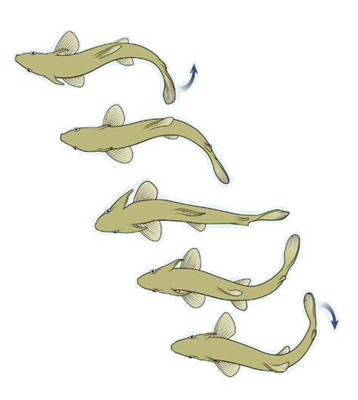
\includegraphics[width=50mm]{motion2.jpg }}
		%
        %\item Calculation of the Buoyancy and weight
        %\item Selection and testing of actuators, communication module and hardware 
        %\item Designing of the control circuits and remote
 
        %Include images/demo of accomplished work
\centering
\fbox{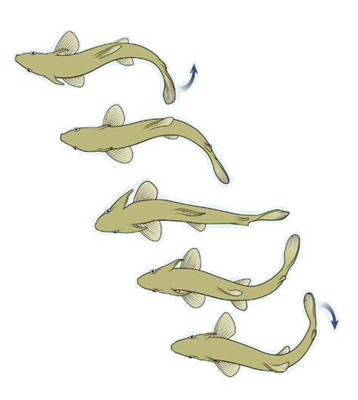
\includegraphics[width=50mm]{motion2}}
\end{frame}

\begin{frame}{Actuation and Motion}
	\fbox{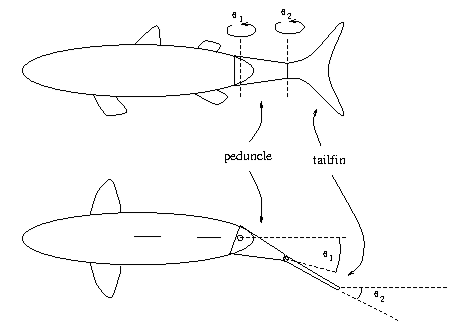
\includegraphics[width=100mm]{motion3}}
\end{frame}

\begin{frame}{Design of the fish}
	\begin{itemize}
    \item 3D Modelling the fish body
    \end{itemize}
     \centering
 \fbox{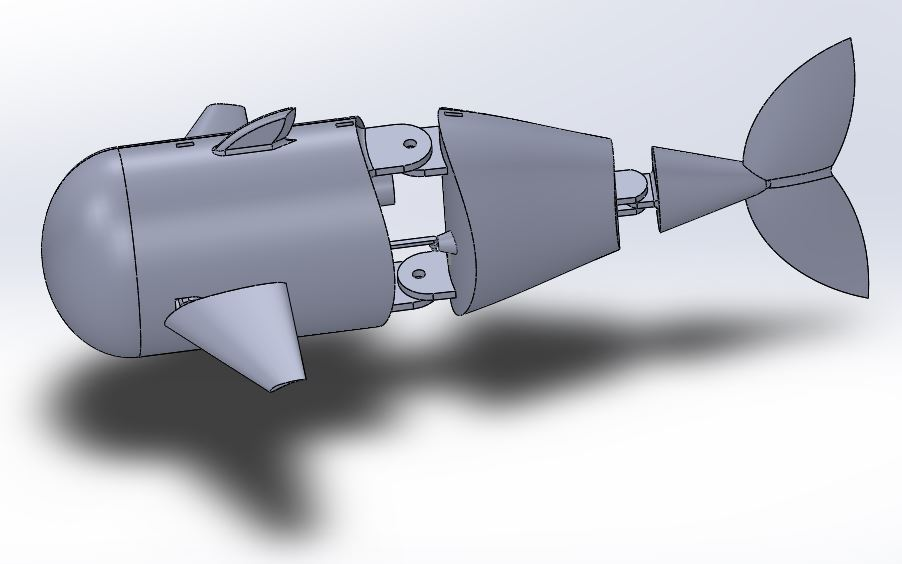
\includegraphics[width=90mm]{fish}}
\end{frame}

\begin{frame}{Sealing of Body}
	\begin{itemize}
    \item Sealing with gaskets and bolts (Front body)
    \end{itemize}
\fbox{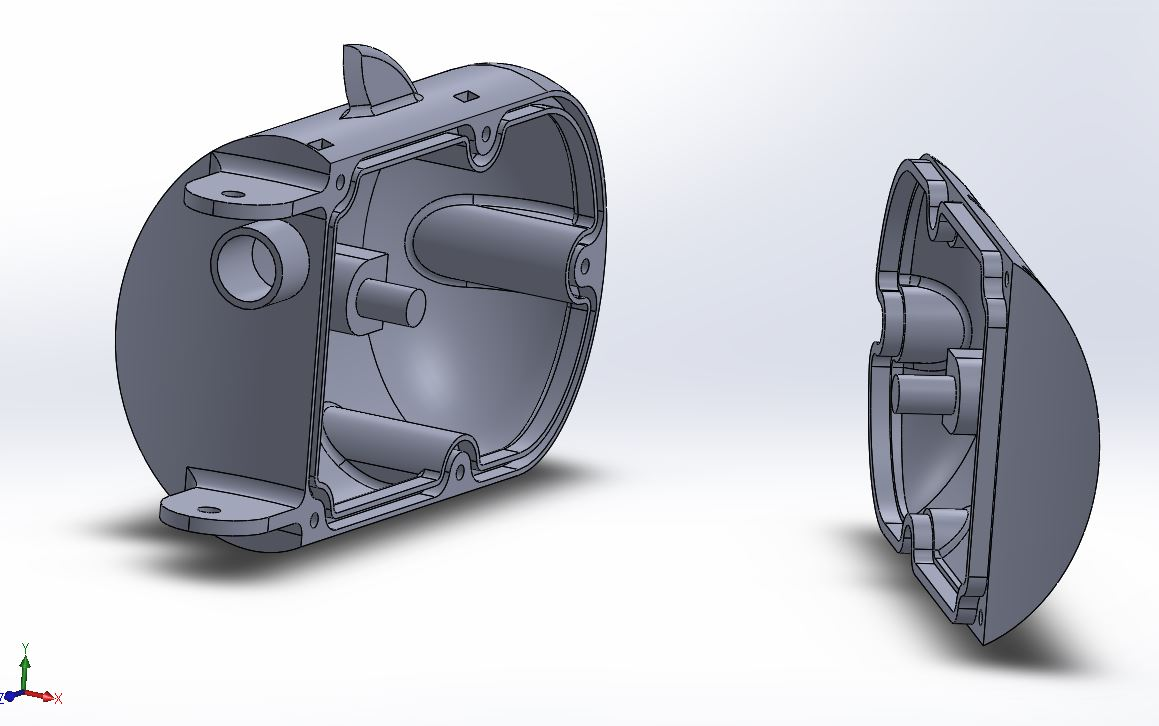
\includegraphics[width=90mm]{fishBody}}
\end{frame}

\begin{frame}{Sealing of Body}
	\begin{itemize}
    \item Modular Body (Midbody)
    \end{itemize}
\fbox{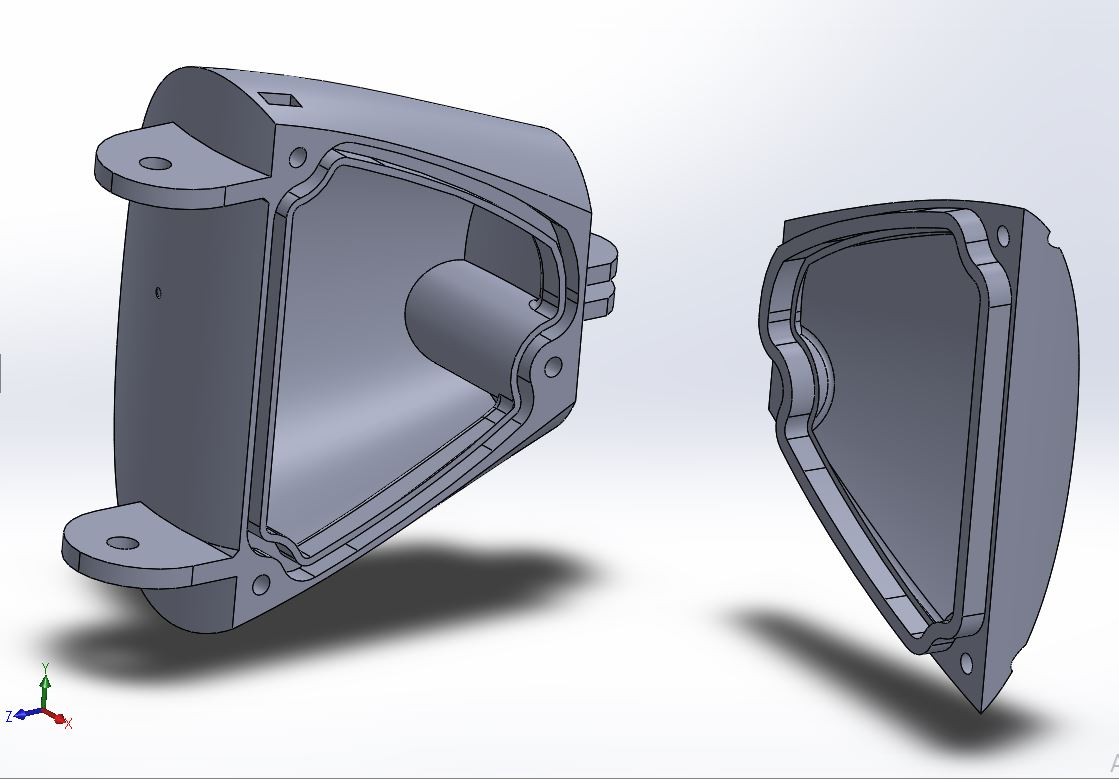
\includegraphics[width=90mm]{fishMiddle}}
%\fbox{\includegraphics[width=90mm]{fishtail}}
\end{frame}

\begin{frame}{A look inside}

\centering
\fbox{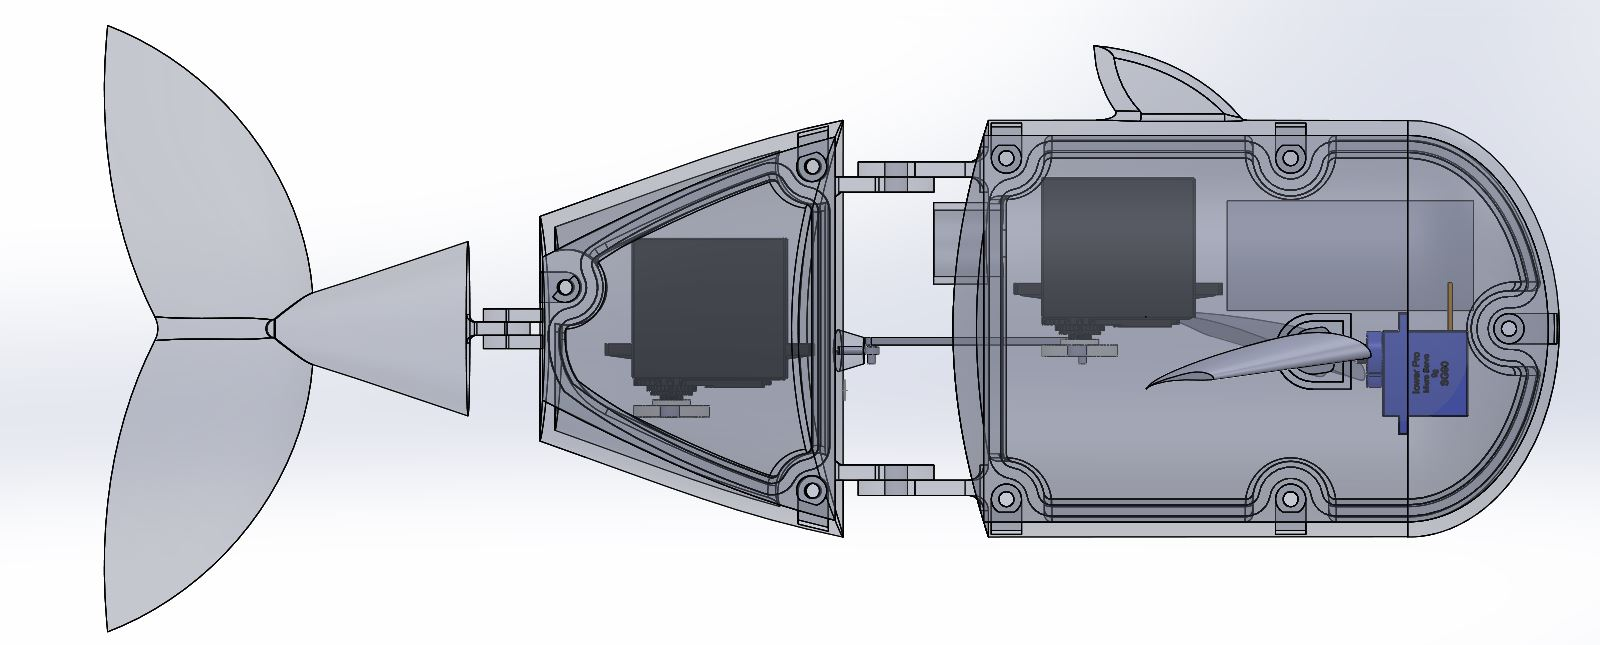
\includegraphics[width=100mm]{fish2}}
\end{frame}

\begin{frame}{The Electronics}
\centering
\fbox{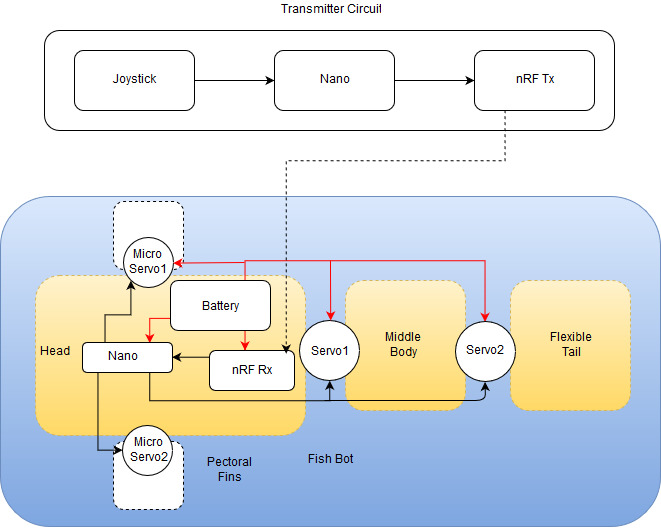
\includegraphics[width=90mm]{blockdia}}	
\end{frame}

\begin{frame}{Electronic components chosen and Why?}
\centering
\begin{itemize}
\setlength\itemsep{1em}
    \item nRF24L01 (2.4 GHz)
    \item Arduino Nano
    \item Reed Switch / Hall sensor
    \item LM338 Regulator
    \item MG958 Servo Motors
    \item 11.1V 1500mAh 30C LiPo Battery
    
    \end{itemize}
%\fbox{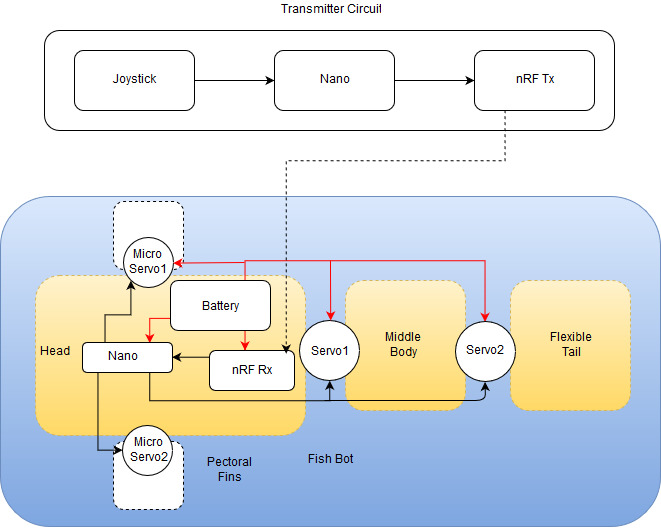
\includegraphics[width=90mm]{blockdia}}	
\end{frame}

\begin{frame}{Designed PCBs}
\begin{itemize}
    \item Controller Board
    \end{itemize}
\centering
\fbox{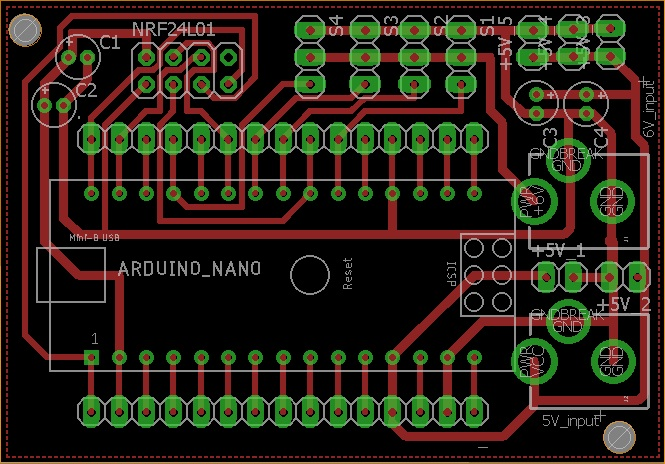
\includegraphics[width=90mm]{ctrl_brd.jpg}}	
\end{frame}

\begin{frame}{Designed PCBs}
\begin{itemize}
    \item Power Supply Board
    \end{itemize}
\centering
\fbox{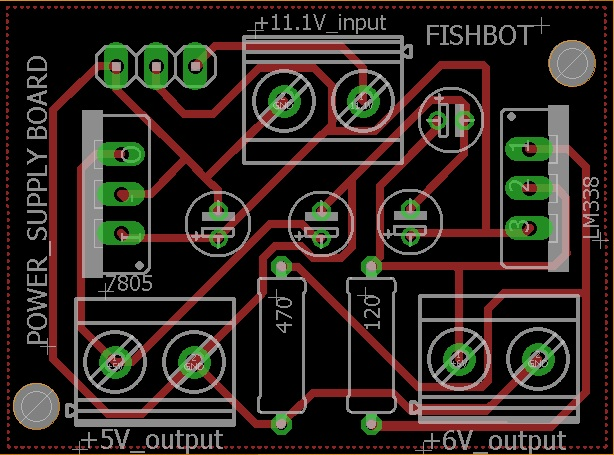
\includegraphics[width=90mm]{power_supply_brd.jpg}}	
\end{frame}


\section{Challenges Faced}
\begin{frame}{Challenges Faced}
	\begin{itemize}
    \setlength\itemsep{1em}
		\item Waterproofing the body
        \item Actuating without waterproof servos
        \item Buoyancy
        \item Maintaining CG and CB 
        \item Underwater communications
        \item Miniaturizing the circuits
	\end{itemize}
\end{frame}

\section{Future Plans}
\begin{frame}{Future Plans}
	\begin{itemize}
    \setlength\itemsep{1em}
        \item Completion of fabrication and assembly of the fish
        \item Integrating the electronics into the fish body
        \item Leak-proofing the fish body and waterproofing the circuits
        \item Testing underwater
	\end{itemize}
\end{frame}

\section{Thank You}
\begin{frame}
	\centering Questions, Queries, Doubts, Suggestions?
\end{frame}

\begin{frame}{Thank You}
	\centering THANK YOU !!!\\
\end{frame}

\end{document}
